\documentclass[pdftex,a4paper,14pt,english,russian]{extarticle}

\usepackage[top=2cm,bottom=27mm,left=3cm,right=18mm]{geometry}
\usepackage[T2A]{fontenc}
\usepackage[utf8]{inputenc}
\usepackage[english,russian]{babel}
\usepackage[pdftex]{hyperref}
\usepackage{indentfirst}
\usepackage[pdftex]{graphicx}
\usepackage{amsmath}
\usepackage{amssymb}
\usepackage{ragged2e}
\usepackage{multirow}
\usepackage{algorithmic}
\usepackage[boxed]{algorithm}
\usepackage{tabularx}
\usepackage{xtab}
\usepackage{subfig}
\usepackage{hyphenat}
\usepackage{setspace}
\usepackage{fancyhdr}

\pagestyle{fancyplain}
\fancyhf{}
\renewcommand{\headrulewidth}{0pt}
\rfoot{\fancyplain{}{\thepage}}

\linespread{1.15}
\floatname{algorithm}{Алгоритм}

\addto\captionsrussian{\renewcommand{\contentsname}{СОДЕРЖАНИЕ}}

\numberwithin{equation}{section}

% new commands
\newcommand\sign[1]{sign(#1)}
\newcommand{\todobiography}{insert biography here}

\begin{document}

\setcounter{page}{1}
\tableofcontents
\newpage

\sectioncentered*{Введение}
\addcontentsline{toc}{section}{Введение}

Целью данного дипломного проекта является разработка алгоритмов машинного обучения, которые позволяют улучшить выдачу поисковых систем. Кроме этого проект демонстрирует как можно использовать неявные пользовательские отзывы(логи сессий) для улучшения ранжирования. 

Поиск информации представляет собой процесс выявления в некотором множестве документов (текстов) всех тех, которые посвящены указанной теме (предмету), удовлетворяют заранее определенному условию поиска (запросу) или содержат необходимые (соответствующие информационной потребности) факты, сведения, данные.

Процесс поиска включает последовательность операций, направленных на сбор, обработку и предоставление информации.

В общем случае поиск информации состоит из четырех этапов:

\begin{itemize}
	\item определение (уточнение) информационной потребности и формулировка информационного запроса
	\item определение совокупности возможных держателей информационных массивов (источников)
	\item извлечение информации из выявленных информационных массивов;
	\item ознакомление с полученной информацией и оценка результатов поиска
\end{itemize}

Информационный поиск — большая междисциплинарная область науки, стоящая на пересечении когнитивной психологии, информатики, информационного дизайна, лингвистики, семиотики, и библиотечного дела.

Поиск информации — процесс выявления в массиве информации записей, удовлетворяющих заранее определенному условию поиска или запросу.

Информационный поиск рассматривает поиск информации в документах, поиск самих документов, извлечение метаданных из документов, поиск текста, изображений, видео и звука в локальных реляционных базах данных, в гипертекстовых базах данных таких, как Интернет и локальные интранет-системы.

Существует некоторая путаница, связанная с понятиями поиска данных, поиска документов, информационного поиска и текстового поиска. Тем не менее, каждое из этих направлений исследования обладает собственными методиками, практическими наработками и литературой.

В настоящее время информационный поиск — это бурно развивающаяся область науки, популярность которой обусловлено экспоненциальным ростом объемов информации, в частности в сети Интернет. Информационному поиску посвящена обширная литература и множество конференций.

В последнее время наблюдается бурное развитие интернета. Количество интернет порталов и сайтов растет с очень большой скоростью и сейчас практически невозможно найти нужную информацию без поисковых систем. В свою очередь, поисковые системы должны отфильтровать и отсортировать огромный объём данных, чтобы предоставить желаемую информацию. Данная задача называется задачей ранжирования. 

Обучение ранжированию — это класс задач машинного обучения с учителем, заключающихся в автоматическом подборе ранжирующей модели по обучающей выборке, состоящей из множества списков и заданных частичных порядков на элементах внутри каждого списка. Частичный порядок обычно задаётся путём указания оценки для каждого элемента (например, «релевантен» или «не релевантен»; возможно использование и более, чем двух градаций). Цель ранжирующей модели — наилучшим образом (в некотором смысле) приблизить и обобщить способ ранжирования в обучающей выборке на новые данные. Это ещё довольно молодая, бурно развивающаяся область исследований, возникшая в 2000-е годы с появлением интереса в области информационного поиска к применению методов машинного обучения к задачам ранжирования.

Для любого алгоритма машинного обучения требуется обучающая выборка. Основной единицей обучения является пара документ-запрос и релевантность документа, данному запросу. Но, в зависимости от алгоритма обучения используются три подхода: 

\begin{itemize}

	\item Поточечный подход. В поточечном подходе предполагается, что каждой паре запрос-документ поставлена в соответствие численная оценка. Задача обучения ранжированию сводится к построению регрессии: для каждой отдельной пары запрос-документ необходимо предсказать её оценку.

	\item Попарный подход. В попарном подходе обучение ранжированию сводится к построению бинарного классификатора, которому на вход поступают два документа, соответствующих одному и тому же запросу, и требуется определить, какой из них лучше.

	\item Списочный подход. Списочный подход заключается в построении модели, на вход которой поступают сразу все документы, соответствующие запросу, а на выходе получается их перестановка. Подгонка параметров модели осуществляется для прямой максимизации одной из перечисленных выше метрик ранжирования.

\end{itemize}

Для построения модели ранжирования, был выбран поточечный подход. В данном дипломном проекте модель ранжирования представляет собой градиентный бустинг на основе решающих деревьев. Для получения релевантности документов из поисковых сессий была применена динамическая байесова сеть

Задача обучения ранжированию на онове кликов нетривиальна. В ~\cite{joachims} было показано, что даже если документы в выдаче отсортированы в обратном порядке(от худшего к лучшему), пользователи будут сначало производить клики по документам, которые занимают первые места. Поэтому, недостаточно просто отсортировать все документы по количеству кликов. В всязи с этим разрабатываются спеуиальные математические модели, которые потом тренируются на обучающей выборке для нахождения релевантности документов.

\newpage
\section{Композиции алгоритмов. Градиентный бустинг}

При решении сложных задач классификации, регрессии, прогнозирования часто оказывается, что ни один из алгоритмов не обеспечивает желаемого качества восстановления зависимости. В таких случаях имеет смысл строить композиции алгоритмов, в которых ошибки отдельных алгоритмов взаимно компенсируются. Наиболее известные примеры композиций — простое и взвешенное голосование. 

\subsection{Композиция алгоритмов}
Введем множество объектов $X$ и множество ответо $Y$. Наряду с этими множествами, введем вспомогательное множество $R$, называемое пространством оценок. Рассматриваются алгоритмы, имеющие вид суперпозиции $a(x)=C(b(x))$, где функция $b: X \to R$ называется алгоритмическим оператором, функция $C: R \to Y$ - решающее правило. 

Многие алгоритмы классификации имеют именно такую структуру: сначала вычисляются оценки принадлежности объекта классам, затем решающее правило переводит эти оценки в номер класса. Значением оценки $b(x)$ может быть вероятность принадлежности объекта x классу, расстояние от объекта до разделяющей поверхности, степень уверенности классификации и т.п.

Введем полное определение классификатора, на основе модели композиции. Композицией $T$ алгоритмов $a_t(x)= C(b_t(x)), t=1,\dotsc,T$ называется суперпозиция алгоритмических операторов $b_t: X \to R$, корректирующей операции  $F: R^T \to R$ и решающего правила $C: R \to Y$:


\begin{equation}
	a(x) = C(F(b_1(x),\dotsc,b_T(x))), x \in X
\end{equation}

Алгоритмы $a_t$, а иногда и операторы $bt$ , называют базовыми алгоритмами. 
Суперпозиции вида $F(b_1,\dotsc, b_T)$ являются отображениями из $X$ в $R$, то есть, опять-таки, алгоритмическими операторами. Это позволяет строить иерархические композиции, применяя определение 1.1 рекурсивно.

Пространство оценок $R$ вводится для того, чтобы расширить множество допустимых корректирующих операций. Можно было бы определить корректирующую операцию и как отображение $F: Y^T \to Y$ , то есть комбинировать непосредственно ответы базовых алгоритмов. Однако в задачах классификации, когда множество $Y$ конечно, число «разумных» корректирующих операций такого вида невелико, что ограничивает возможность оптимизации $F$ под конкретную задачу \todobiography. Если же ком бинировать ответы алгоритмических операторов, то операция $F$ получает на входе оценки принадлежности объекта классам — более точную информацию, не огрублённую решающим правилом.

\subsection{Взвешанное голосование}

Корректирующая операция $F$ может иметь параметры, настраиваемые по обучающей выборке, наряду с параметрами базовых алгоритмов. Например, в линейной комбинации настраиваются веса $at$ базовых алгоритмов:

\begin{equation}
	b(x)=F(b_1(x), \dotsc ,b_T(x)) = \sum_{t=1}^{T} a_tb_t(x),  x \in X,  a_t \in R
\end{equation}

Если веса $a_t$ неотрицательны и нормированы, $\sum_{t=1}^{T} a_t =1$ , то композицию (1.2) называют выпуклой комбинацией базовых алгоритмов. Естественно предполагать, что вес $a_t$ тем больше, чем выше качество базового алгоритма $b_t$.

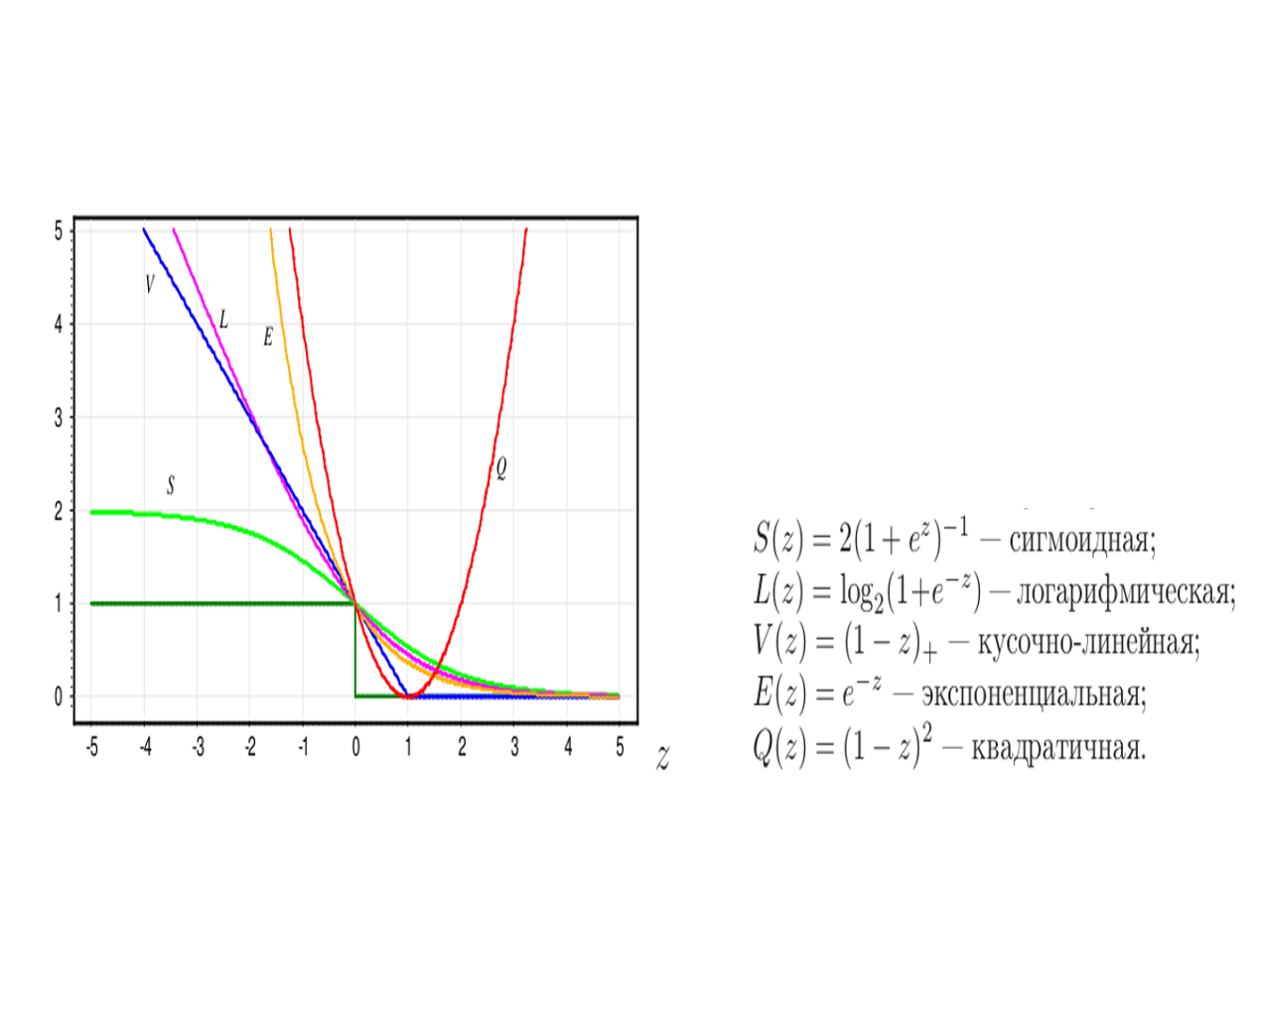
\includegraphics[width=0.9\textwidth]{images/upper_approximations.png}

\subsection{Бустинг}

Построение бустинга лучше всего рассматривать на задаче для двух классов ${-1,1}$, а потом обобщить на общий случай, для множества классов $M$. Пусть есть двух классовая задача $Y={-1,+1}$. Допустим, что решающее правило фиксировано, $C(b) = sign(b)$, базовые алгоритмы возвращают ответы $-1,0,+1$. Ответ $b_t(x) = 0$ означает, что базовый алгоритм $b_t$ отказывается от классификации объекта $x$, и ответ $b_t(x)$ не учитывается в композиции.
Искомая алгоритмическая композиция имеет вид:
\begin{equation}
	a(x)=C(F(b_1(x),\dotsc,b_T(x)))=sign(\sum_{t=1}^{T} a_tb_t(x)), x \in X
\end{equation}

Определим функционал качества композиции как число ошибок, допускаемых
ею на обучающей выборке:
\begin{equation}
	Q_T=\sum_{t=1}^{l} y_i\sum_{t=1}^{T} a_tb_t < 0]
\end{equation}

Напрямую, оптимизировать такой функционал очень сложно, поэтому заменим его на оценку сверху:
\begin{equation}
	Q_T=min_{\beta_m,\gamma_m}\sum_{i=1}^{N}L(y_i,\sum_{m=1}^{M}\beta_m b(x_i;\gamma_m)))
\end{equation}
В качестве функции потерь $L(y_i,f_m(x;\gamma)$ могут выступать функции, приведенные на рисунке 1.
Общий алгоритм бустинга:

\begin{algorithm}
  \caption{Общий алгоритм бустинга}
  \label{overall-boosting-algorithm}
  \begin{enumerate}
  \item Инициализировать переменные $f_0(x)=0$
  \item Для каждого шага $m=1,2 .. M$:
    \begin{enumerate}
      \item Вычисляем $(\beta_m,\gamma_m)=arg \min_{\beta,\gamma} \sum_{i=1}^{N}L(y_i,f_{m-1}(x_i)+\beta b(x_i;\gamma))$
      \item $f_m(x)=f_{m-1}(x)+\beta_m b(x;\gamma_m)$
    \end{enumerate}
  \end{enumerate}
\end{algorithm}



\begin{algorithm}
  \caption{Градиентный бустинг для многоклассовой классификации}
  \label{gradient-boosting-algorithm}
  \begin{enumerate}
  \item Инициализировать переменные $f_0(x)=0, k=1,2,...,K$
  \item Для каждого шага $m=1,2 .. M$:
    \begin{enumerate}
      \item Вычислить:
      \begin{equation}
      	p_k(x)=\frac{e^{f_k(x)}}{\sum_{l=1}^{K}e^{f_l(x)}}, k=1,2,...,K
      \end{equation}
      \item Для k = 1 до K:
      \begin{enumerate}
      	\item $r_{ikm}=y_{ik}-p_k(x_i), i=1,2,...,N$, где $y_{ik}=1$ если $y_i$ принадлежит классу $k$, иначе 0.
      	\item Для множества пар $(x_i,r_ikm)$ построить решающее дерево. С конечными регионами: $R_{jkm}, j=1,2,...,J_m$
      	\item $\gamma_{jkm}=\frac{K-1}{K}\frac{\sum_{x_i\in R_{jkm}}r_{ikm}}{\sum_{x_i\in R_{jkm}}|r_{ikm}|(1-|r_{ikm}|})$
      	\item Обновить $f_{km}=f_{k,m-1}(x)+\sum_{j=1}^{J_m}\gamma_{jkm}I(x\in R_{jkm}$
      \end{enumerate}
    \end{enumerate}
    \item Выход: $f_k=f_{km}(x), k=1,2,...,K$
  \end{enumerate}
\end{algorithm}

\end{document}

